This chapter evaluates the process of designing secure mobile applications using SKF and the final results.

\section{Discussion}
SKF has proven to be partially successful in the secure SDLC of developing CheFeed. It has shown that it can generate security requirements based on the projects needs. Furthermore, based on the requirements we come to understand what potential security risks are introduced for the development of the user authentication and user session management feature which is useful during the design phase of the SDLC. 

Design however does not always directly translate into code implementation. This can be due to a lack of understanding of the programming language or the level of security training the developer has received. Not all security requirements were implemented by the developing team. Furthermore, a lack of security training and understanding of implementing security tests made the testing phase difficult. Even with the security testing guide and mappings provided by SKF, without proper education and training it is still difficult to understand how static analysis tools are to be used for security specifically. Although the MSTG and its test cases provide detailed explanation, they are technical and do require further research into the recommended static analysis tools and dynamic analysis tools. Therefore, this study mainly resolved to manual code reviews. Table \ref{tab:results-implemented} describes what security controls have been implemented during development of CheFeed for both the API and client-side.

\begin{table}[!b]
    \centering
    \caption{Results implemented security controls}
    \label{tab:results-implemented}
    \begin{tabulary}{1.0\textwidth}{|L|l|}
        \hline
        \textbf{Security Control} & \textbf{Implemented} \\
        \hline
        System credential storage facilities need to be used to store sensitive data, such as PII, user credentials or cryptographic keys & Yes \\
        \hline
        No sensitive data should be stored outside of the app container or system credential storage facilities & No \\
        \hline
        No sensitive data is written to application logs & Yes \\
        \hline
        The keyboard cache is disabled on text inputs that process sensitive data & No \\
        \hline
        No sensitive data, such as passwords or pins, is exposed through the user interface & Yes \\
        \hline
        If the app provides users access to a remote service, some form of authentication, such as username/password authentication, is performed at the remote endpoint & Yes \\
        \hline
        If stateless token-based authentication is used, the server provides a token that has been signed using a secure algorithm & Yes \\
        \hline
        The remote endpoint terminates the existing session when the user logs out & Yes \\
        \hline
        A password policy exists and is enforced at the remote endpoint & Yes \\
        \hline
        Sessions are invalidated at the remote endpoint after a predefined period of inactivity and access tokens expire & Yes \\
        \hline
        Authorization models should be defined and enforced at the remote endpoint & Yes \\
        \hline
    \end{tabulary}
\end{table}

\section{Test Results}
The static analysis tools on both the API repository and client side repository were added to continuous integration pipeline. Figure \ref{} shows the test results for the API. The figure shows that for the API one medium severity finding was one found. Here it concerns a security misconfiguration where the secret key is hard coded in the source code.

Although the client side repository had semgrep added to the continous integrated pipeline, it had difficulties in finalizing the scanning progress as seen in figure \ref{}.

\begin{figure}
    \centering
    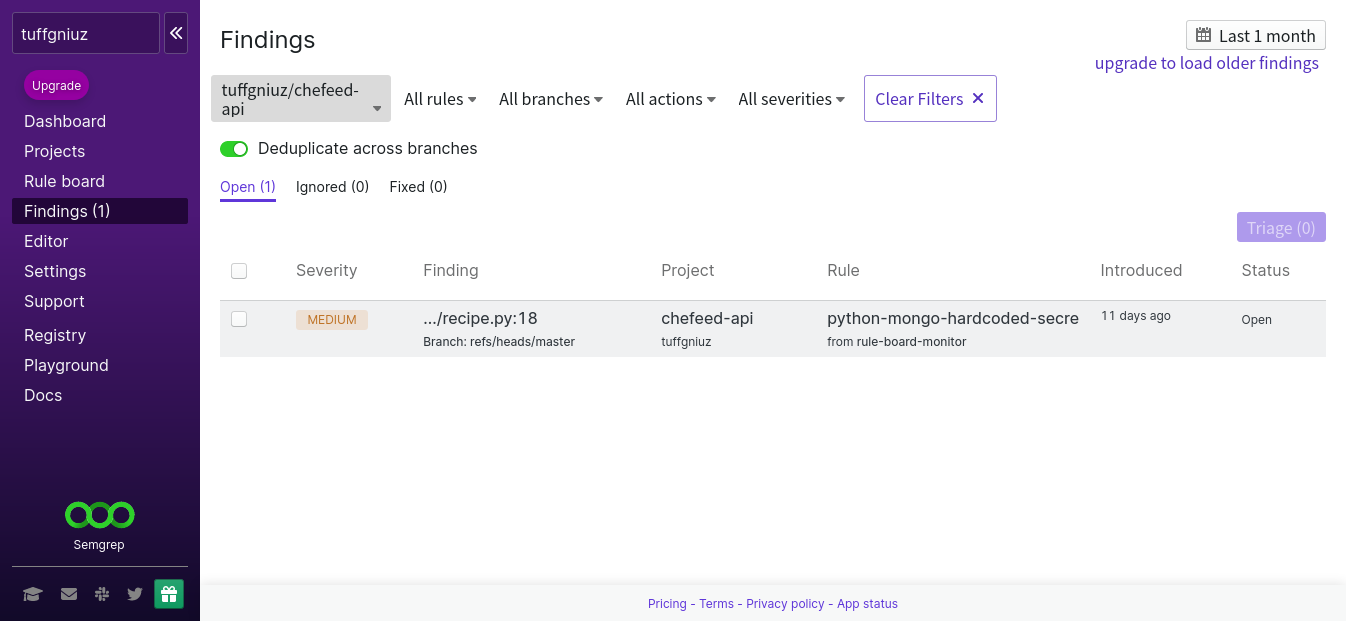
\includegraphics[width=\textwidth]{chapter-6/api-semgrep-results}
    \caption{SEMGREP results for the API}
    \label{fig:api-semgrep}
\end{figure}

\begin{figure}
    \centering
    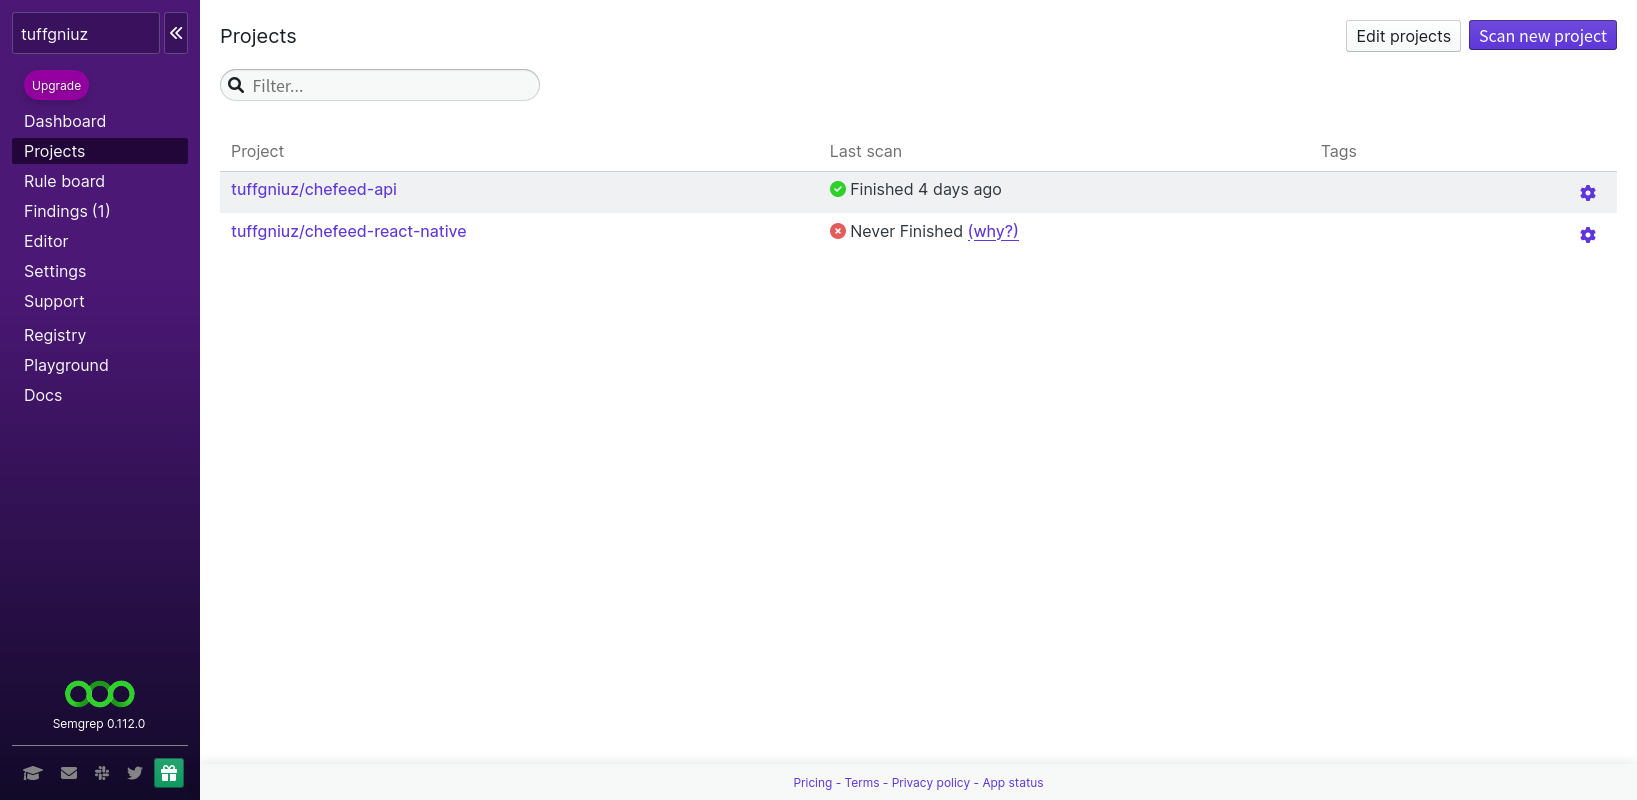
\includegraphics[width=\textwidth]{chapter-6/semgrep-failed}
    \caption{Failed scan on the client side code}
    \label{fig:failed-semgrep-scan}
\end{figure}


